\subsubsection{Event}
\begin{figure}[h]
	\centering
	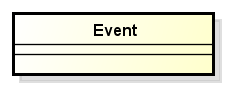
\includegraphics[width=0.5\linewidth]{img/premi_back_end_event}
	\caption[Diagramma della classe Event]{Diagramma della classe Event}
	\label{fig:premi_back_end_event}
\end{figure}


\paragraph{Descrizione}
La classe Events è una classe astratta che viene estesa da tutti i nuovi eventi creati.

\newpage
\subsubsection{ProjectWasCreated}
\begin{figure}[h]
	\centering
	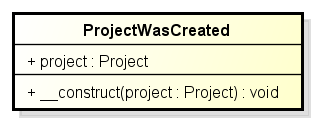
\includegraphics[width=0.5\linewidth]{img/premi_back_end_project_was_created}
	\caption[Diagramma della classe ProjectWasCreated]{Diagramma della classe ProjectWasCreated}
	\label{fig:premi_back_end_project_was_created}
\end{figure}


\paragraph{Descrizione}
La classe ProjectWasCreated è un evento che gestisce la creazione di un nuovo progetto, creando una presentazione con prima slide di default ad esso correlato.

\paragraph{Utilizzo}
Utilizzata quando viene creato un nuovo progetto.

\paragraph{Attributi}
\begin{itemize}
	\item \textbf{+ project : Project}\\
	Variabile di istanza che contiene il progetto che ha generato l'evento.   
\end{itemize}

\paragraph{Metodi:}
\begin{itemize}
	\item \textbf{+ \_\_construct(project: Project) : void}\\
	Crea una nuova istanza dell'evento:\\
	\textbf{Argomenti:}
	\begin{itemize}
		\item project : Project;
		Progetto che ha scatenato l'evento.
	\end{itemize}
\end{itemize}